\section{Methodology}

\begin{figure}[tb]
    \begin{minipage}{0.48\textwidth}
      \centering
      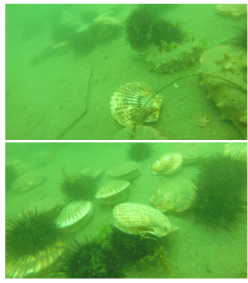
\includegraphics[width=.7\linewidth]{figures/pre-processing.png}
      \label{Fig:PreProcessing}
    \end{minipage}\hfill
    \begin{minipage}{0.48\textwidth}
      \centering
      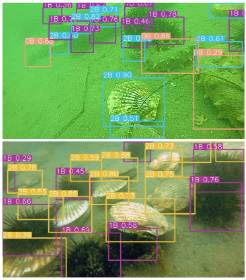
\includegraphics[width=.7\linewidth]{figures/post-processing.png}
      \label{Fig:PostProcessing}
    \end{minipage}
    \caption{Pre-processing and Post-processing of underwater images (\cite{jiangUnderwaterSpeciesDetection2021})}
\end{figure}

\subsection{Data Collection}

In this project, publicly available underwater image datasets with labels about
underwater species will be used, as these are more prevalent and accessible.
Specifically, the datasets to be used include the Underwater Object Detection Dataset (UODD)
\parencite{jiangUnderwaterSpeciesDetection2021}\footnote{UODD dataset is available at \url{https://github.com/LehiChiang/Underwater-object-detection-dataset}},
and the Brackish Dataset introduced by \Textcite{pedersenDetectionMarineAnimals2019}
\footnote{Brackish Dataset is available at \url{https://www.kaggle.com/aalborguniversity/brackish-dataset}}.
These datasets contain a diverse range of underwater scenes,
including various species such as fish, crabs, and starfish,
providing a comprehensive basis for testing and comparison. The annotations are labeled
in formats like MS COCO, facilitating consistent and detailed evaluation of model performance.

\subsection{Image Pre-Processing}

Pre-processing of images plays a crucial role in enhancing the quality and clarity of underwater images,
which can significantly impact the performance of deep learning models.
The following techniques will be used and tested to improve image quality:

\begin{itemize}
    \item \textbf{Image Enhancement}: Techniques such as histogram equalization and contrast adjustment will be used to improve the visibility of features in underwater images.
    \item \textbf{Noise Reduction}: Methods like median filtering and Gaussian blur will be applied to reduce the noise inherent in underwater images.
    \item \textbf{Color Correction}: Algorithms such as white balance adjustment and color channel compensation will be utilized to correct the color distortions caused by underwater lighting conditions.
    \item \textbf{Normalization}: Pixel values will be normalized to a standard range to ensure consistency across the dataset, facilitating better learning and generalization by the models.
\end{itemize}

\subsection{Model Selection and Development}

\begin{APAitemize}
    \item \textbf{CNNs}: Initial experiments will focus on conventional
     Convolutional Neural Networks (CNNs), which have proven effective in basic underwater object
     detection tasks \parencite{hanUnderwaterImageProcessing2020}. 
     CNNs utilize layers of convolutional filters to extract features from images. 
     Mathematically, a convolution operation on an image \( I \) with a filter \( K \) 
     is defined as:
     \begin{equation}
     (I * K)(x,y) = \sum_{i=-m}^{m} \sum_{j=-n}^{n} I(x+i, y+j) K(i, j)
     \end{equation}
     where \( (x, y) \) are the coordinates of the pixel \parencite{dumoulinGuideConvolutionArithmetic2018}.
     These models will serve as a benchmark for comparing more advanced architectures.

    \item \textbf{Residual Networks (ResNets)}: Given their ability to train
     deeper networks by mitigating the vanishing gradient problem \parencite{heDeepResidualLearning2016},
     ResNets will be explored for their potential to improve recognition accuracy in complex underwater scenes.
     ResNets introduce shortcut connections that skip one or more layers, which helps in addressing the vanishing gradient problem. 
     The residual block can be expressed as:
     \begin{equation}
     y = F(x, \{W_i\}) + x
     \end{equation}
     where \( x \) is the input to the residual block, \( F \) is the residual mapping, and \( \{W_i\} \) are the weights of the layers in the block \parencite{heDeepResidualLearning2016}. This allows the network to learn the residual mapping instead of the original unreferenced mapping.

     \item \textbf{Transformers}: The study will also incorporate Transformer
     models \parencite{hanSurveyVisionTransformer2023}, which utilize self-attention mechanisms to examine their
     effectiveness in capturing the spatial relationships of objects in underwater images.
     The self-attention mechanism computes a weighted sum of input features, where the weights are determined by the similarity between elements.
     Given an input sequence of vectors \( X = [x_1, x_2, \ldots, x_n] \), the self-attention mechanism is defined as:
     \begin{equation}
     \text{Attention}(Q, K, V) = \text{softmax}\left(\frac{QK^T}{\sqrt{d_k}}\right)V
     \end{equation}
     where \( Q \) (queries), \( K \) (keys), and \( V \) (values) are linear transformations of \( X \), and \( d_k \) is the dimension of the key vectors \parencite{vaswaniAttentionAllYou2023}. This mechanism allows the model to weigh the importance of different elements in the sequence dynamically.
\end{APAitemize}

\subsection{Implementation}

The project will employ Python as the primary programming language,
leveraging its extensive ecosystem and the ease of finding pre-implemented
models along with Jupyter notebook to help the visualization of data.
For model implementation and training, I will utilize deep learning
libraries such as TensorFlow and PyTorch. TensorFlow and PyTorch offer extensive support for building and training deep learning models, including pre-built layers, optimization algorithms, and GPU acceleration.

Experiments will be conducted on a laptop equipped with an Nvidia GPU
to facilitate efficient model training and evaluation.
The GPU acceleration is critical for handling the computational load of training
deep learning models, as it significantly speeds up the process by performing parallel computations.

\subsection{Evaluation Criteria}

The evaluation of the various models will use common indicators like accuracy, precision,
recall, and F1 score to determine the effectiveness of each model in correctly
identifying and classifying underwater objects.

\begin{itemize}
    \item \textbf{Accuracy}: This measures the overall correctness of the model, defined as the ratio of correctly predicted instances to the total instances.
    \begin{equation}
    \text{Accuracy} = \frac{TP + TN}{TP + TN + FP + FN}
    \end{equation}

    \item \textbf{Precision}: This measures the accuracy of the positive predictions, defined as the ratio of true positive instances to the total predicted positive instances.
    \begin{equation}
    \text{Precision} = \frac{TP}{TP + FP}
    \end{equation}

    \item \textbf{Recall}: This measures the ability of the model to identify all relevant instances, defined as the ratio of true positive instances to the total actual positive instances.
    \begin{equation}
    \text{Recall} = \frac{TP}{TP + FN}
    \end{equation}

    \item \textbf{F1 Score}: This is the harmonic mean of precision and recall, providing a single metric that balances both. It is defined as:
    \begin{equation}
    F1 = \frac{2 \times \text{Precision} \times \text{Recall}}{\text{Precision} + \text{Recall}}
    \end{equation}
\end{itemize}

Additionally, computational efficiency, measured in terms of training time and inference speed, will be considered to assess the practicality of deploying these models in real-world applications. Computational efficiency is crucial as it impacts the feasibility of using these models in environments with limited computational resources or in scenarios requiring real-time processing.

The performance of each architecture will be compared to establish their relative strengths and weaknesses in underwater object recognition. This analysis will also explore the impact of varying dataset complexities and environmental conditions on model performance.


\FloatBarrier

% TODO: Improve methodology, add more info about how the evaluation will take place, mode formulas maybe? 